% "Shadow maps and projective texturing in X3D" by Michalis Kamburelis,
% accepted for Web3D 2010.
%
% © Copyright 2010 by ACM, Inc.
% See http://www.acm.org/publications/policies/copyright_policy
%

%% Template stuff begins here ------------------------------------------------

\documentclass{acmsiggraph}                     % final
%\documentclass[annualconference]{acmsiggraph}  % final (annual conference)
%\documentclass[review]{acmsiggraph}            % review
%\documentclass[widereview]{acmsiggraph}        % wide-spaced review
%\documentclass[preprint]{acmsiggraph}          % preprint

\usepackage[scaled=.92]{helvet}
\usepackage{times}
\usepackage{graphicx}
\usepackage{parskip}
\usepackage[labelfont=bf,textfont=it]{caption}
\onlineid{1010} %% I think this doesn't matter

%% Template stuff ends here ------------------------------------------------

% This is really the only sensible way to make breaking of monospace text
% (everything inside \texttt, including (but not limited) to urls).
% Otherwise, the monospace text flows outside of the column all over the place.
\sloppy

\usepackage{needspace}

%% For href
\usepackage{ifpdf}
\ifpdf
  \usepackage[pdftex]{hyperref}
\else
  \usepackage[hypertex]{hyperref}
\fi

%% Put float in a nice box,
%% http://en.wikibooks.org/wiki/LaTeX/Floats,_Figures_and_Captions
\usepackage{float}
\floatstyle{boxed}
\newfloat{mycodecore}{H}{listofmycode}
\floatname{mycodecore}{}

% Fix mycodecore: it has additional vertical line at the bottom after the frame.
% Possibly due to Verbatim inside?
\newenvironment{mycode}
{\begin{mycodecore}}
{\end{mycodecore}
\vspace{-0.1in}}

%% Use verbatim that allows \latex commands inside,
%% highly useful for my node spec figures.
%% See http://scott.sherrillmix.com/blog/category/programmer/latex/,
%% http://www.ctan.org/tex-archive/macros/latex/contrib/fancyvrb/
\usepackage{fancyvrb}

%% To allow tex_projected at the bottom.
%% Without this, figure* can only go to the top (or separate page).
%% http://en.wikibooks.org/wiki/LaTeX/Floats,_Figures_and_Captions#Wide_figures_in_two_column_documents
\usepackage{stfloats}

%% Bold inside our code/spec samples.
%%
%% For an older acm style (from
%% http://www.acm.org/sigs/publications/proceedings-templates)
%% this was a hack:
%% we get some strange teletype font that cannot be bold (it just looks
%% the same). It's a pity, since my verbatims really depend on bold parts
%% for good look. Workaround was to just resign from teletype.
%%
%% For acm siggraph from http://www.siggraph.org/publications/instructions/index.html
%% this simply makes text bold, no tricks.
\newcommand*{\codeem}[1]{\textbf{#1}}

% \nolinkurl is a trick to allow links to break across lines in pdf,
% from http://www.miwie.org/tex-refs/html/latex-packages.html#hyperref
\newcommand*{\myhref}[2]{\texttt{\href{#1}{\nolinkurl{#2}}}}

% The above \myhref unfortunately (due to \nolinkurl trick)
% makes it impossible to break links manually.
% So below is the same as \myhref, but does not break link text automatically,
% and allows to break it manually (by inserting \\ etc.)
% \newcommand*{\myhrefm}[2]{\texttt{\href{#1}{#2}}}

\newenvironment{myenumerate}
{\begin{enumerate}
  \setlength{\itemsep}{0pt}
  \setlength{\parskip}{0pt}
  \setlength{\parsep}{0pt}}
{\end{enumerate}}

\title{Shadow maps and projective texturing in X3D}

\author{Michalis Kamburelis\thanks{e-mail: michalis.kambi@gmail.com}\\Institute of Computer Science\\University of Wroc{\l}aw, Poland}
%% no full addr here, I think?
%% ul. Joliot-Curie 15
%% 50-383 Wroc{\l}aw, Poland

\keywords{X3D graphics, shadows, shadow maps, projective texturing}

\begin{document}

\teaser{
  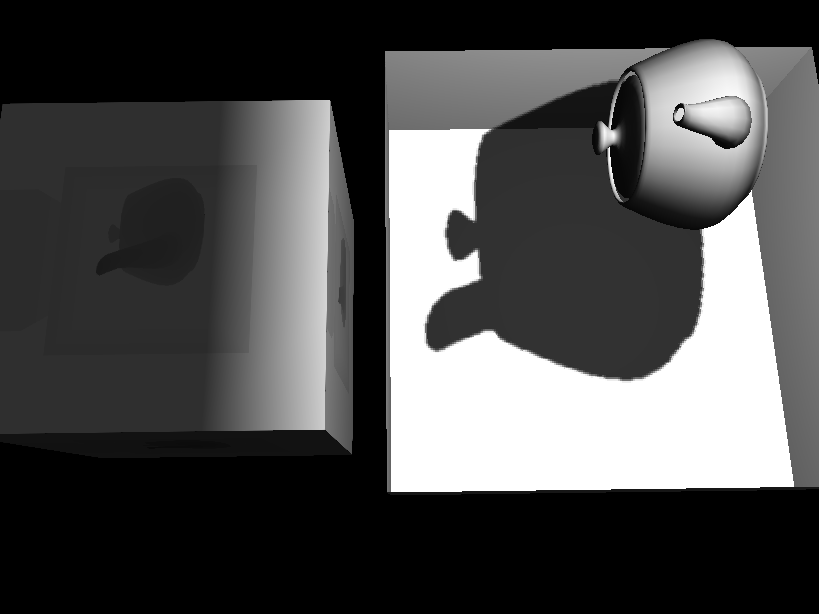
\includegraphics[width=2.19in]{simple_shadow_map_teapots}
%  \caption{Teapot casting a shadow. On the left, a direct view of it's shadow map is visible. Shadow maps rendered.}
  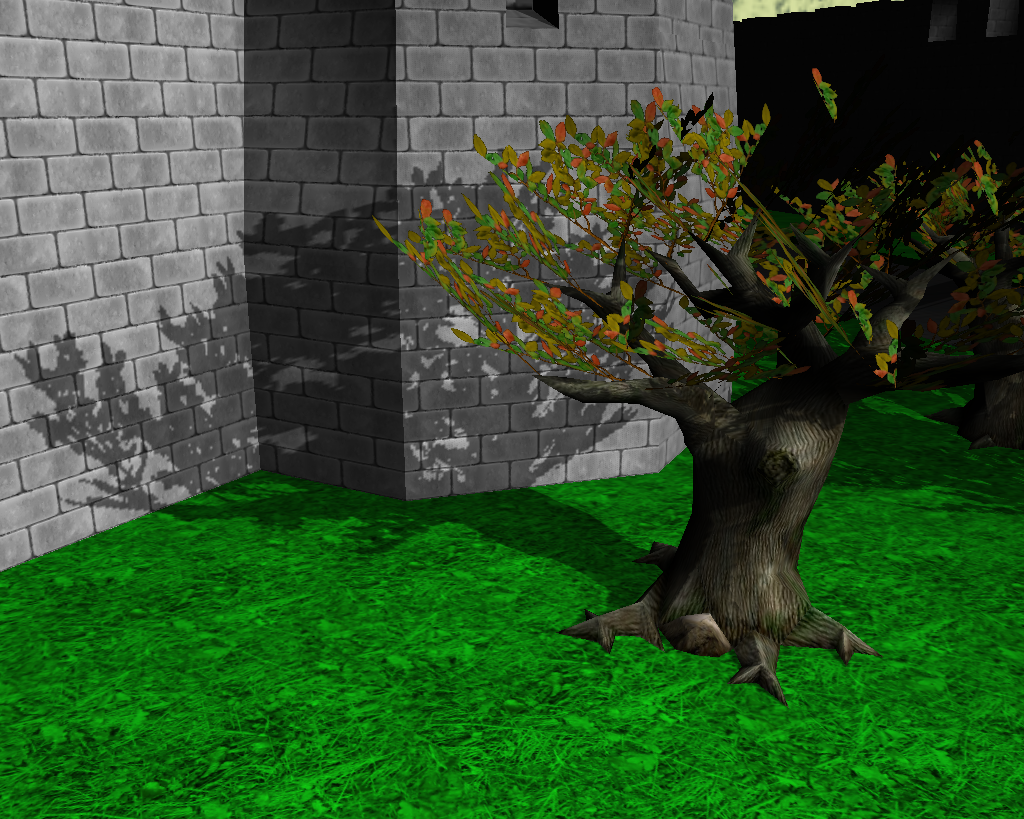
\includegraphics[width=2.19in]{sunny_street_tree_hard_tall}
  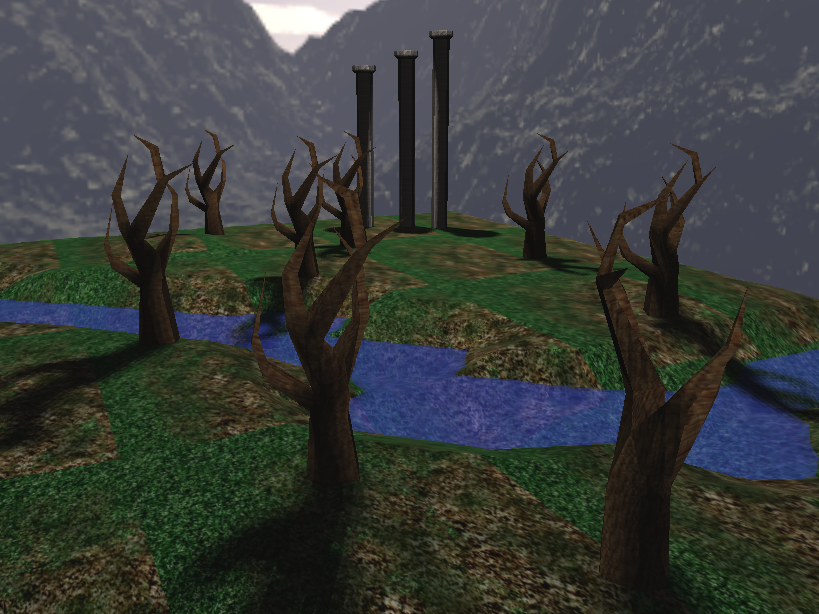
\includegraphics[width=2.19in]{trees_river_shadow_maps}
%  \caption{Trees and columns casting a shadow.}
}

\maketitle

\begin{abstract}
We propose a number of X3D extensions to enable shadows in the virtual worlds.
Our higher-level extensions are an easy way to request shadows
independently of their implementation.
Lower-level extensions allow to control the details of
\emph{shadow maps} generation and \emph{projective texture mapping}.
Together, they allow the authors to activate real-time dynamic shadows
on 3D scenes. The extensions expose also projective texture mapping
for purposes other than shadows, for example we can cast a color texture
from a light source. Introduced concepts map naturally to any basic
shadow maps implementation,
and integrate nicely with existing X3D components like textures and shaders.
\end{abstract}

\begin{CRcatlist}
  \CRcat{I.3.7}{Computer Graphics}{Three-Dimensional Graphics and Realism}{Color, shading, shadowing, and texture};
  \CRcat{I.3.6}{Computer Graphics}{Methodology and Techniques}{Languages, Standards}
\end{CRcatlist}

\keywordlist

%% \terms{Languages, Standardization, Algorithms}
%% not needed with acmsiggraph template?

\section{Introduction}

%% The ``\copyrightspace'' command must be the first command after the
%% start of the first section of the body of your paper. It ensures the
%% copyright space is left at the bottom of the first column on the first
%% page of your paper.
\copyrightspace

X3D \cite{x3d:spec} is an open standard for representing rich 3D data.
Many advanced graphic effects are available for the creators of interactive
3D worlds.
% Authors can even use custom GPU shader code.

\emph{Shadow maps} \cite{sm} are one of the major approaches for generating
real-time dynamic shadows. They are relatively simple to implement,
supported by graphics hardware (both in fixed-function pipeline and shaders),
and with proper implementation can achieve very good quality.
They work with any geometry, including difficult cases like
3D geometry that is not correctly closed,
flat 2D geometry and alpha-test textures.
They have no problems with dynamic environments.

A closely related subject is \emph{projective texturing} \cite{nvidia:proj}.
It is utilized by the shadow maps algorithm, but is useful also
in other circumstances, when you want to ,,cast'' a texture from a light.

In this paper we introduce a number of X3D extensions to
use and control shadow mapping and projective texturing.
Our extensions allow the authors of virtual worlds to easily use shadow maps
in the scene. They also expose the most useful shadow mapping parameters,
so that they can be tuned to achieve the best results.
Authors also get control over projective texturing, that may be used
with any kind of textures --- like depth textures generated by shadow maps,
the standard color textures, and any other texture types
expressible in X3D.

Authors that attach shaders to the geometry (for example using
the OpenGL Shading Language, GLSL) get explicit control over
what happens with the shadow map values. This allows to use our shadow maps
in non-trivial scenarios, combining them with a custom shading methods and such.
Also \emph{percentage closer filtering} \cite{gpugems:pcf}
can be trivially implemented inside the shader.

For the developers of X3D browsers, our extensions strive to be relatively easy to implement.
Any basic shadow maps implementation should naturally map to presented new nodes
and fields. An example open-source implementation, supporting all
the extensions' features, is available inside the VRML/X3D engine
on \myhref{http://vrmlengine.sourceforge.net/}{http://vrmlengine.sourceforge.net/}.

\section{Shadow maps algorithm}
\label{sec_algorithm}

For the purpose of better understanding the following extensions,
we present here a short overview how shadow mapping works.
This is intentionally a simplified overview, implementors will most
definitely want to look at more detailed articles like
NVidia presentations \cite{nvidia:sm}, \cite{nvidia:hsm}. Shadow maps are
suitable for implementation in both OpenGL, Direct3D, and in software renderers.

%% Relevant OpenGL extensions' specifications are \texttt{ARB\_shadow}
%% \cite{glext:shadow} and \texttt{ARB\_depth\_texture}
%% \cite{glext:depthtexture} (available as part of the \emph{core} since
%% OpenGL 1.4).
%% Wikipedia page \myhref{http://en.wikipedia.org/wiki/Shadow\_mapping}{http://en.wikipedia.org/wiki/Shadow\_mapping}
%% (as of 2010-04-21) also presents a nice overview of the subject with many
%% useful references.

\needspace{1in}
The first step is to \textbf{generate the shadow map texture}.
We place the camera at the position of a light source, and point it in the
light's direction. Then we render the depth buffer of the scene to
a \emph{depth texture}. This step must be done before rendering the actual
scene with shadows.

\begin{figure}[H]
  \centering
  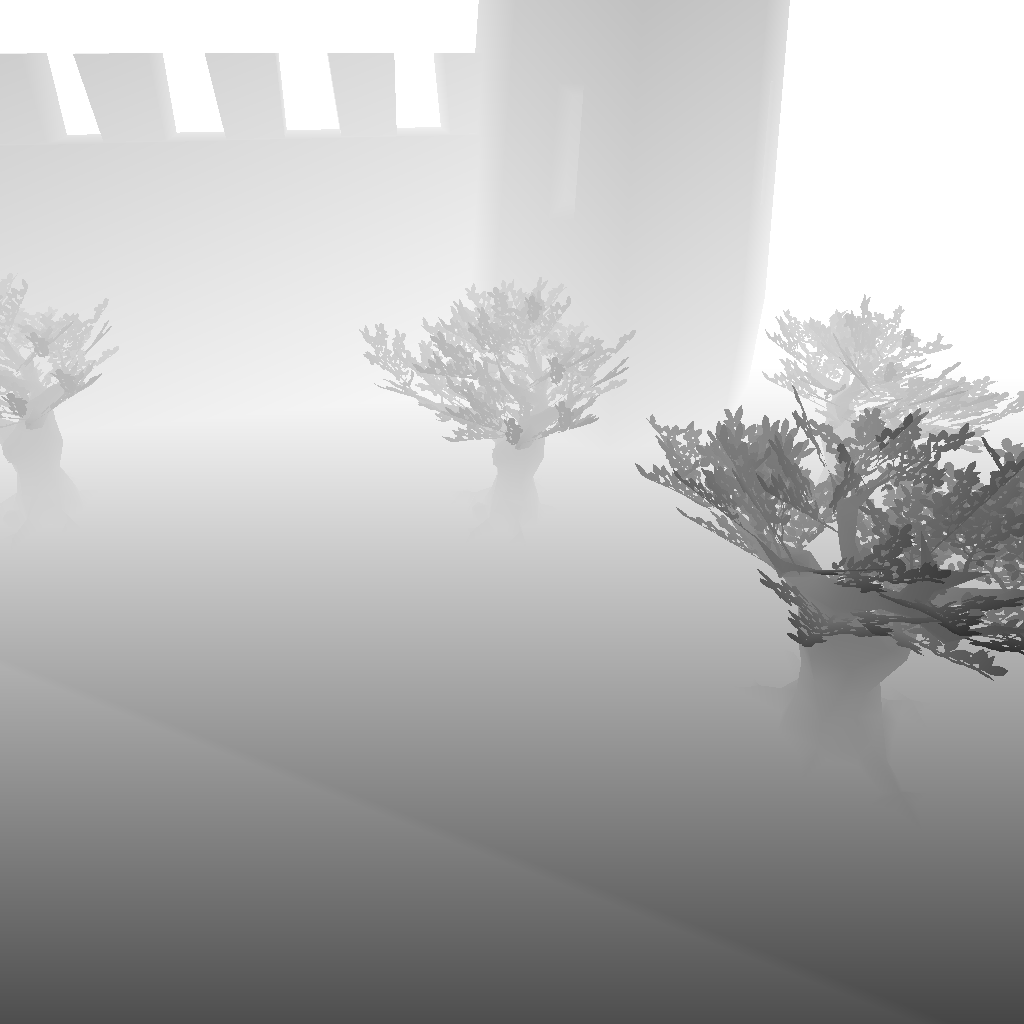
\includegraphics[width=3in]{depths_light_mapped}
  \caption{Shadow map, as seen from the light source. Darker colors mean that the object is closer to the light source.}
\end{figure}

Since a point light source doesn't have a direction, a common solution
is to render \emph{six} depth textures along the six major directions
(-/+X, -/+Y, -/+Z, usually in the global coordinate space). This way we map
the view around an imagined cube around the light source.

For a directional light source, we need to know its position.
Although conceptually directional light is positioned at infinity,
for shadow maps we must assign a normal 3D position even to a directional light.
Together with the projection near and far plane, this position is needed to determine
what depths will be captured accurately, that is which shadow casters
will cast a correct shadow.

For light sources that have parallel rays (like a directional light),
we use orthographic projection. For others (like a positional or spot light)
we use perspective projection.

Once we have a shadow map, the second step is to
\textbf{map the generated texture on shadow receiving geometry}.
This is done during the normal rendering of the scene, when the camera
corresponds to the avatar view. We want to map the texture treating
the light source like a projector that ,,casts'' the texture onto the scene.
This stage of the algorithm is known as the \emph{projective texturing},
and can be used as well for other purposes, like projecting standard color
textures over the scene.

Knowing the lights projection parameters and the current
camera parameters we want to calculate the texture coordinate $t$
for a point $p$ like

\begin{equation}
  t = S * L_p * L_v * C_v^{-1} * p
\end{equation}

Where $L_p$ is the light projection matrix, $L_v$ is the light view
matrix, and $C_v$ is the camera (representing the avatar)
view matrix. $S$ is a trivial constant matrix to scale and shift clip coordinates
by $\frac{1}{2}$, to have the texture coordinates in $[0..1]$ range.

\begin{figure}[H]
  \centering
  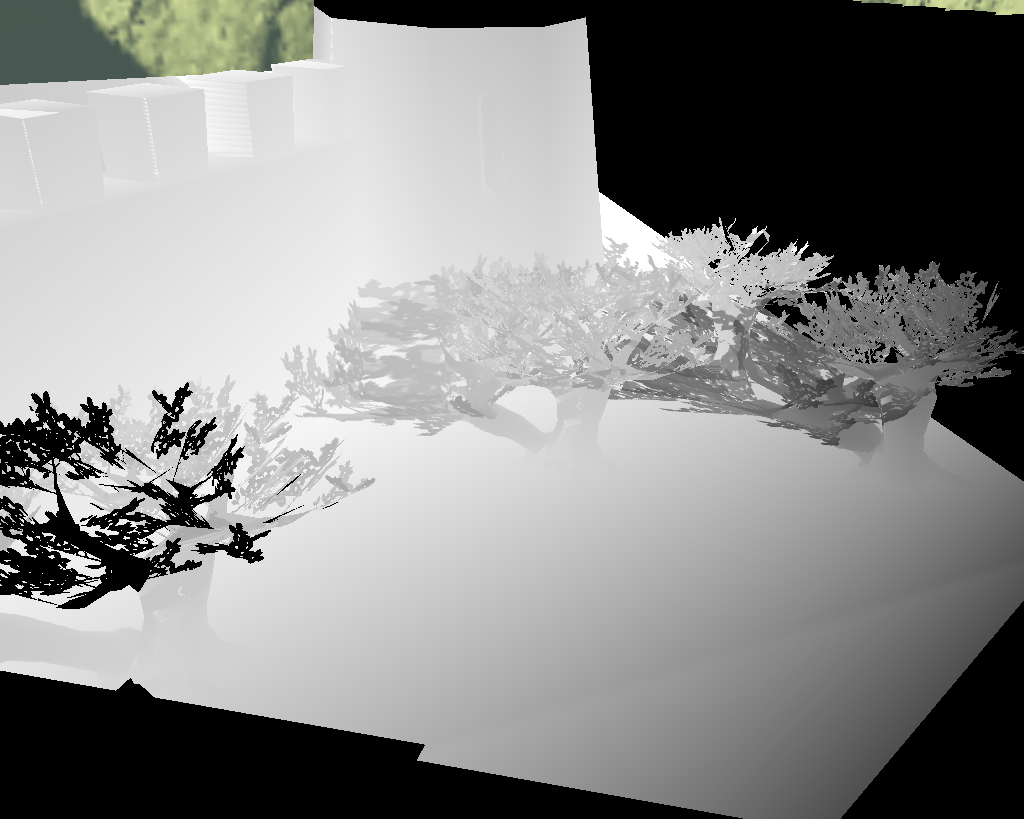
\includegraphics[width=3in]{depths_camera_mapped}
  \caption{Shadow map, as seen from the avatar camera. This is the previous shadow map projected over the scene.}
\end{figure}

Calculated $(t.x, t.y)$ can be used to sample the shadow map,
to get the distance from the light to the object that obscures the light
source at this point. Calculated $t.z$ contains the distance from the light
to the current point. Thus the third and final step is to
\textbf{determine if the point lies in the shadow} by comparing

\begin{equation}
  t.z > texture(shadowMap, t.x, t.y)
\end{equation}

Note that in 3D graphics we use 4x4 matrices,
and 3D positions are expressed in the 4D homogeneous coordinates.
The vectors after perspective transformation will have the 4th component ($t.w$)
different than $1$, so this cannot be ignored.
So the real equation is actually

\begin{equation}
  \frac{t.z}{t.w} > texture(shadowMap, \frac{t.x}{t.w}, \frac{t.y}{t.w})
\end{equation}

For simplicity, let's call $t.z/t.w$ simply a $d$ (for \textit{distance to the point}).

When the object is not in the shadow, $d$ is equal to the texture value
(we're looking at the object obscuring the light).
Otherwise, it's larger (we're looking at the object \emph{behind} the one obscuring the light).
In a perfect world (assuming an infinite resolution of the shadow map,
no floating point errors etc.) $d$ should never be smaller than the right side
of the equation.

Careful reader will notice now that the world is not actually perfect.
Precision of the depth values is limited,
and gets worse the farther away from the light source we are.
The shadow map resolution never matches perfectly the
screen resolution (one shadow map pixel may correspond to many screen pixels).
And finally we have to account for the floating point calculation errors.
Due to these problems, a small offset
is needed to make the comparison with $d$ above behave stable.
Our extensions encourage the implementation to apply this offset when generating
the shadow map, and allow the author to adjust the offset parameters
for particular cases.

At the end we want to actually use the results of the above comparison.
That is, we want to \textbf{render the places in shadow with darker colors}.
In the simplest case, we can simply make the surface black when
it is in the shadow or use the original color when surface is lit.
This step is controlled fully in the shader, so shader authors may
apply here any shading algorithm they see fit.

\section{Overview and discussion}

Many scene elements cooperate to produce a nice shadow effect: light
sources, shadow casters and shadow receivers. This enables various
potential ways for spreading the shadow information over the X3D
nodes. Our extensions put the main weight on the \emph{shadow
receivers}. You have to explicitly designate shapes receiving
the~shadow: either by the simple \texttt{Appearance.receiveShadows} field,
or by using the lower-level tools \texttt{GeneratedShadowMap},
\texttt{ProjectedTextureCoordinate} and custom shaders.

Specifying additional shadow information at the light sources and
shadow casters is purely optional. Every light source may cast
shadows, and everything is a shadow caster by default.

Compare this with other approaches by BS~Contact
\cite{bs:72}, \cite{bs:62} and Octaga \cite{octaga:shadow}. Their approaches
favor specifying shadow information in separate nodes (\texttt{Shadow}
in Octaga, \texttt{ShadowGroup} in BS Contact) that explicitly
enumerate shadow casters (occluders, emitters) and receivers.

Both Octaga and BS Contact provide also lower-level nodes for
storing the shadow maps (\texttt{ShadowTexture} in Octaga, for BS Contact
this is a special case of \texttt{CompositeTexture3D}). This is
analogous to our \texttt{GeneratedShadowMap} node and serves a similar
purpose: author can get more control over shadow mapping this way.
In particular, custom fragment shaders may be used to visualize shadows.
%% However, there is no analogy to our \texttt{ProjectedTextureCoordinate}
%% as far as we know (it can be simulated by performing the calculating the appropriate
%% matrix is script), and no analogy to our \texttt{Appearance.shadowCaster} field.

Various needs guided the design of our shadow extensions:

\begin{enumerate}
\itemsep 0pt
\item \textbf{Flexibility of what casts and receives the shadow}. In the
  extreme case, we could specify on each shadow receiver from
  which lights it receives shadow, and for every combination of light and
  shadow receiver --- which shapes occlude the light. We think
  this is too burdensome for typical uses, and stands in the direct
  opposition to the goal of \textbf{easily enabling shadows on the
  existing scenes}.

  Our extensions allow to choose only lights on the shadow
  receivers. Configuration of shadow casters is global, that is an
  object either casts a shadow on all the shadow receivers, or doesn't
  cast a shadow at all.

\item \textbf{Flexibility of what shadow method is used}. Our
  extensions, as well as BS Contact and Octaga, are strongly directed at the
  shadow mapping algorithms. Our extensions are also usable for other
  shadow approaches, as long as the author uses only the most
  encouraged \texttt{Appearance.receiveShadows} and the
  \texttt{Appearance.shadowCaster} extensions.

  The important point here
  is that our \texttt{receiveShadows} field can work really well,
  so many scenes are fine using it
  and thus work with any shadow algorithm.

\item \textbf{Natural behavior for authors}. Not much technical
  knowledge should be required from the authors, and the shadow
  properties should be declared where they feel most natural. We think
  that our choice of extending the shadow receivers is the most
  natural here --- receiving the shadow changes the look of given
  shape.

  We also note that this nicely fits with \textbf{natural placement
  for implementors}. In case of shadow maps, receiving the shadows
  requires shading the object differently.
\end{enumerate}

Now that we summarized what we want, let's quickly review where
we can place shadow information in the X3D scene:

\begin{enumerate}
\itemsep 0pt
\item Completely \textbf{separate} nodes, like a special \texttt{Shadow}
  node, do not encourage authors to use shadows widely.

\item Requiring much configuration of the \textbf{shadow casters}
  seems unnecessary, because most shadows algorithms easily account
  for a large number of shadow casters. This is true for shadow maps,
  as well as shadow volumes and ray testing. The only exception could
  be plane-projected shadows, but these depend heavily on the number
  of shadow receivers as well.

  So the best treatment of shadow casters is to make everything, by
  default, a shadow caster, and do not require any configuration for
  them. Algorithms that are internally unable to cope with some shadow
  casters can simply ignore them. For example, shadow volumes
  implementations using classic silhouette optimization may want to
  detect and ignore shapes that are not 2-manifold.

\item Placing information at \textbf{light sources} is natural, and
  our extensions put some information there.

  For shadow algorithms that, in their basic implementation,
  make everything a shadow receiver (like multi-pass shadow volumes,
  or shadow ray testing), it would be possible to make everything a
  shadow receiver by default (and thus, do not require any shadow
  receivers configuration). This could be a working solution for
  small, simple scenes. But for large scenes, we need more flexibility
  to limit the shadows.

\item Thus, the explicit configuration of \textbf{shadow receivers} seems
  like a best choice for us. It is flexible, and still simple enough
  to be widely used on many shapes in the scene. Authors just add
  lights to the \texttt{Appearance.receiveShadows} field in the
  simplest case.

  Moreover, receiving shadows changes the look of the given
  shape. This is a very practical insight, because it means that usage
  of shaders on shadow receivers is limited. For shadow maps, shadow
  receiver must use the appropriate shader. When using the
  \texttt{receiveShadows} field, author must be aware that browser may force
  usage of internal shaders. When placing
  \texttt{GeneratedShadowMap} on the \texttt{textures} list the author
  must be aware that he must write his own shader to
  get really nice shading results.

  %% Admittedly, this decision is related to the shadow maps
  %% algorithm. For other algorithms, for example shadow volumes
  %% implemented as a multi-pass technique, it's easy to treat
  %% everything as shadow receiver. An extension of the light node
  %% that explicitly says "everything receives shadows from this
  %% light" is possible.
\end{enumerate}

\section{X3D extensions}

We present now the actual X3D extensions to enable shadow maps
and projective texturing. We propose to add a couple of new fields
to the existing nodes, and some new nodes.

\needspace{1in}
The specification of nodes and fields in this section is similar to the
X3D specification conventions:

\begin{Verbatim}[commandchars=\\\{\},frame=single]
FieldType [in,out] \codeem{fieldName} <default value>
  # optional range of allowed values
  # for the field above
\end{Verbatim}

\subsection{Define shadow receivers}
\label{sec_receive_shadows}

In the simplest case, to enable the shadows authors must only
use this field:

\begin{mycode}
\underline{New field for the Appearance node}
\begin{Verbatim}[commandchars=\\\{\}]
MFNode  []  \codeem{receiveShadows}  []
  # [X3DLightNode] list
\end{Verbatim}
\end{mycode}

Each light present in the \texttt{receiveShadows} list will cast shadows on
the given shape. That is, contribution of the light source
will be scaled down if the light is occluded at a given fragment.
%% . For the simplest hard shadows implementations,
%% the light contribution will be set to zero (when the light is occluded)
%% or left as is (when light is not occluded).
The whole light contribution is affected, including the ambient term.
%% \footnote{We scale also the ambient term, this way we cooperate easily with
%% lights \texttt{attenuation}, \texttt{on} and \texttt{radius} behavior.
%% In particular, the shadow receiver outside the light's radius is obviously
%% always in the shadow. This way there's no uncertainty whether we should
%% add it's ambient term --- no.}
We do not make any additional changes to the X3D lighting model.
The resulting fragment color is the sum of all the visible lights (visible
because they are not occluded, or because they don't cast shadows on this shape),
modified by the material emissive color and fog, following the X3D specification.

This is the simplest extension to enable shadows.
It is suitable for any shadows implementation, not only shadow maps.

Authors should note that browsers may use internal shaders to produce nice
shading for shadow receivers. Custom author shaders may be ignored.
If you want to apply your own shaders over shadow receivers, you have to
use the lower-level nodes described next instead of this.

\subsection{Overview of the lower-level extensions}

The following extensions make it possible to precisely setup and control
shadow maps. Their use requires a basic knowledge of the shadow map approach,
and they are necessarily closely tied to the shadow map workflow.
On the other hand, they allow the author to define custom shaders
for the scene and control every important detail of the shadow mapping process.

These lower-level extensions give a complete and flexible system to
control the shadow maps, making the \texttt{receiveShadows}
feature only a shortcut for the simplest setup.

We make a shadow map texture by the \texttt{GeneratedShadowMap} node,
and project it on the shadow receiver by
\texttt{ProjectedTextureCoordinate}.
%% When generating and projecting shadow maps we also want to indicate
%% the light source, which in most cases should be the same light source
%% indicated by the X3D \texttt{USE LightName} construct.
An example X3D code (in classic encoding) for a shadow map setup:

\begin{Verbatim}[commandchars=\\\{\},frame=single]
DEF MySpot SpotLight \{
  location 0 0 10
  direction 0 0 -1
  \codeem{projectionNear 1}
  \codeem{projectionFar 20}
\}

Shape \{
  appearance Appearance \{
    texture \codeem{GeneratedShadowMap \{}
      \codeem{light USE MySpot}
      \codeem{update "ALWAYS"}
    \codeem{\}}
  \}
  geometry IndexedFaceSet \{
    texCoord \codeem{ProjectedTextureCoordinate \{}
      \codeem{projector USE MySpot}
    \codeem{\}}
    # ... other IndexedFaceSet fields
  \}
\}
\end{Verbatim}

%% # every Shape in the scene is a shadow caster
%% # by default

\subsection{Light sources parameters}
\label{sec_light_params}

\begin{figure*}[t]
  \centering
  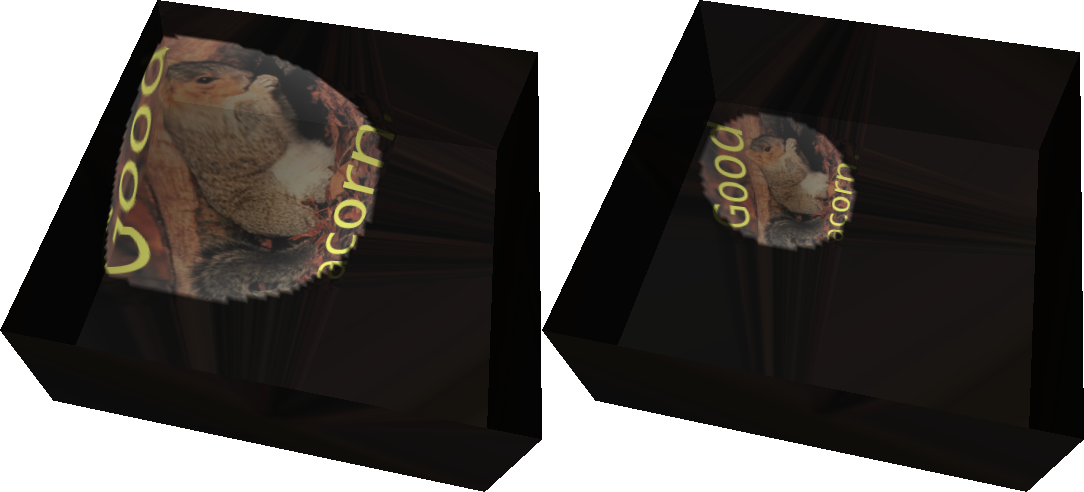
\includegraphics[width=7in]{tex_projected_spot}
  \caption{Spot light cone angle matching with the projected texture angle}
  \label{fig_tex_projected_spot}
\end{figure*}

The motivation behind the extensions in this section is that we want to use
light sources as cameras. This means that lights need additional parameters
to specify projection details.

\needspace{0.5in}
To every X3D light node (\texttt{DirectionalLight}, \texttt{SpotLight},
\texttt{PointLight}) we add new fields:

\begin{mycode}
\underline{Additional fields for every X3DLightNode}
\begin{Verbatim}[commandchars=\\\{\}]
SFFloat  [in,out]  \codeem{projectionNear} 0
  # must be >= 0
SFFloat  [in,out]  \codeem{projectionFar} 0
  # must be > projectionNear, or = 0
SFVec3f  [in,out]  \codeem{up} 0 0 0
SFNode   []        \codeem{defaultShadowMap}  NULL
  # [GeneratedShadowMap]
\end{Verbatim}
\end{mycode}

The fields \texttt{projectionNear} and \texttt{projectionFar} specify the near
and far values for the projection used when rendering to the shadow map texture.
These are distances from the light position, along the light direction.
You should always try to make \texttt{projectionNear} as large as possible
and \texttt{projectionFar} as small as possible,
this will make depth precision better (keeping \texttt{projectionNear} large
is more important for this). At the same time, your projection range
must include all your shadow casters.

The field \texttt{up} is the ,,up'' vector of the light camera when capturing
the shadow map. This is used only with non-point lights
(\texttt{DirectionalLight} and \texttt{SpotLight}).
Although we know the direction of the light source,
but for shadow mapping we also need to know the ,,up'' vector to have camera
parameters fully determined.
This vector must be adjusted by the implementation to be perfectly orthogonal
to the light direction, this allows user to avoid explicitly giving
this vector in many cases. Results are undefined only if this vector
is (almost) parallel to the light direction.

These properties are specified at the light node, because both
shadow map generation and texture coordinate calculation must know them,
and use the same values (otherwise results would not be of much use).

The field \texttt{defaultShadowMap} is meaningful only when some
shape uses the \texttt{receiveShadows} feature. This will be described
in the later section \ref{sec_how_receive_shadows_maps}.

\texttt{DirectionalLight} gets additional fields to specify orthogonal
projection rectangle (projection XY sizes) and location for
the light camera. Although directional light is conceptually at infinity
and doesn't have a location, but for making a texture projection
we actually need to define the light's location.

\begin{mycode}
\underline{Additional fields for the DirectionalLight node}
\begin{Verbatim}[commandchars=\\\{\}]
SFVec4f  [in,out]  \codeem{projectionRectangle}
  0 0 0 0 # left, bottom, right, top;
  # must be left < right and bottom < top,
  # or all zero
SFVec3f  [in,out]  \codeem{projectionLocation}  0 0 0
  # affected by node's transformation
\end{Verbatim}
\end{mycode}

\needspace{1in}
\texttt{SpotLight} gets additional field to explicitly specify a perspective
projection angle.

\begin{mycode}
\underline{Additional fields for the SpotLight node}
\begin{Verbatim}[commandchars=\\\{\}]
SFFloat  [in,out]  \codeem{projectionAngle}  0
\end{Verbatim}
\end{mycode}

Leaving \texttt{projectionAngle} at the default zero value is equivalent
to setting \texttt{projectionAngle} to \texttt{2 * cutOffAngle}.
This is usually exactly what is needed.
Note that the \texttt{projectionAngle} is
the vertical and horizontal field of view for the square texture,
while \texttt{cutOffAngle} is the angle of the half of the cone
(that's the reasoning for $*2$ multiplier).
Using \texttt{2 * cutOffAngle} as \texttt{projectionAngle}
makes the perceived light cone fit nicely inside the projected
texture rectangle. It also means that some texture space is essentially
wasted --- we cannot perfectly fit a rectangular texture into a circle shape.

\begin{figure*}[t]
  \centering
  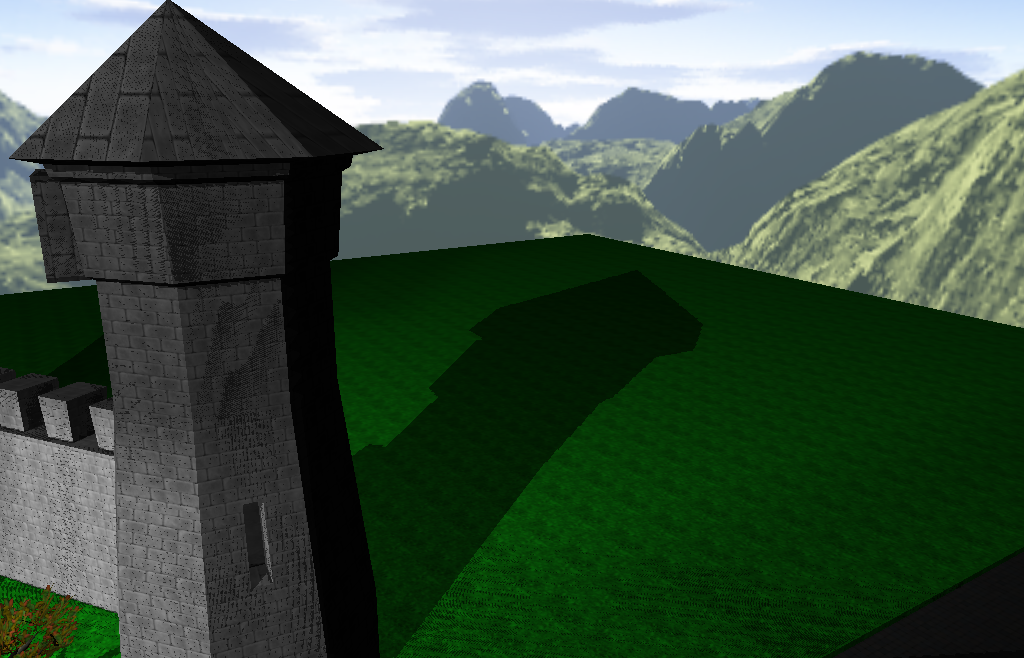
\includegraphics[width=2.2in]{scale_bias_too_small}
  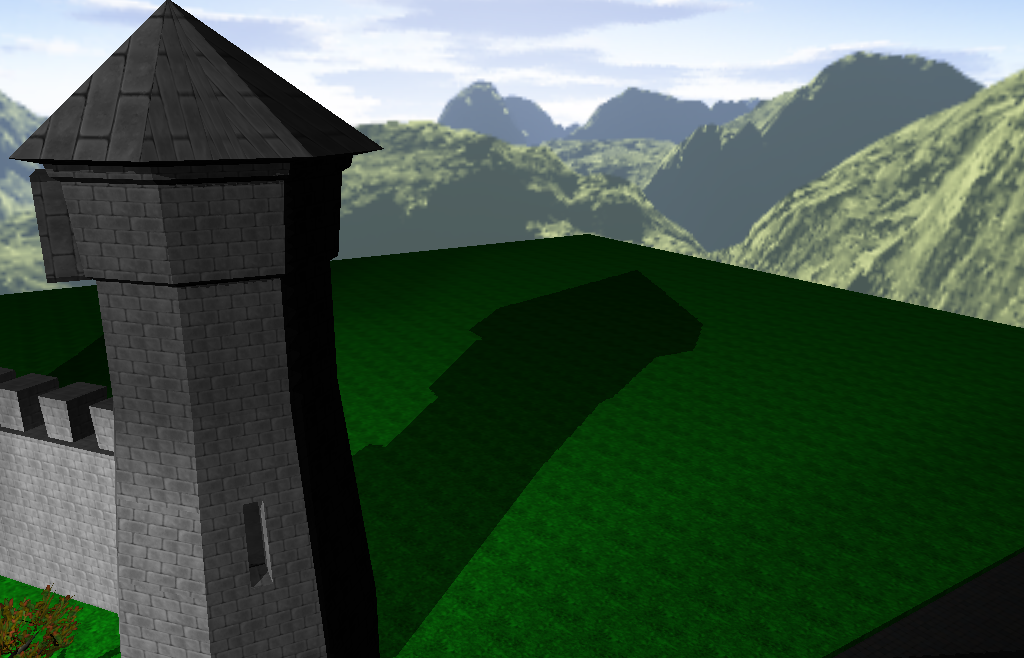
\includegraphics[width=2.2in]{scale_bias_right}
  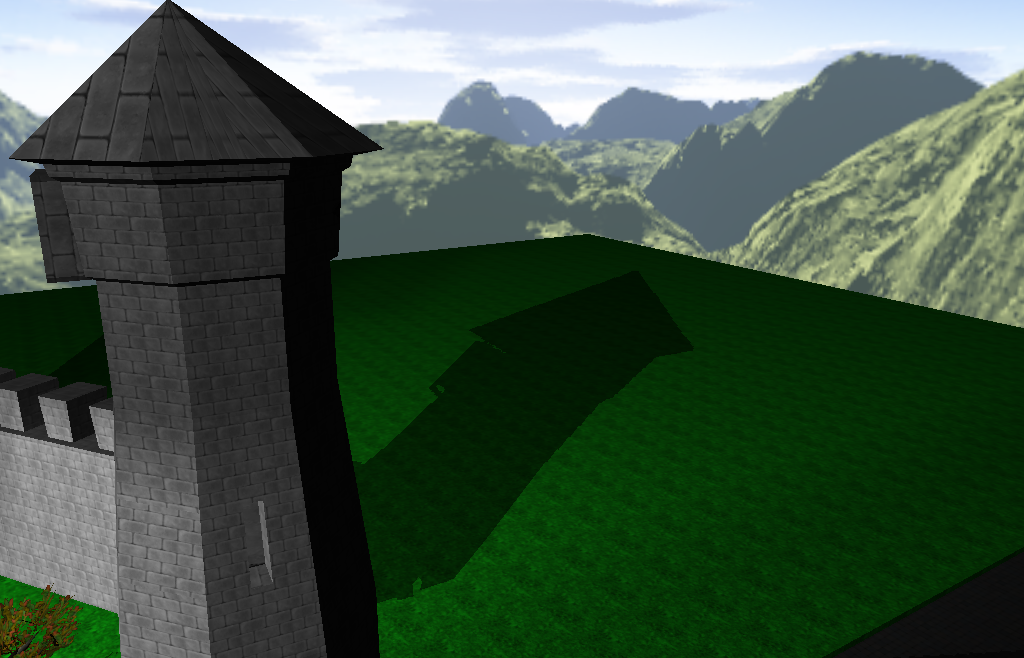
\includegraphics[width=2.2in]{scale_bias_too_large}
  \caption{Various bias/scale values.
On the left, they are too small and the shadow caster is erroneously considered to cast shadow on itself (notice the noise on the tower).
On the right, they are too large and the shadow is pushed back and shrunk (notice how it doesn't touch precisely the bottom of the tower).
In the middle, they are just right (use default values).}
  \label{fig_scale_bias}
%% For demo puposes these screenshots show really
%% extremal values: left is scale = bias = 0, right is scale = bias = 100,
%% middle is the default.
\end{figure*}

Figure \ref{fig_tex_projected_spot} shows how a light cone fits within
the projected texture.

\vspace{-1in} % HACK! To make the damn pagebreak nicely.

\needspace{1in}
\subsection{Automatically generated shadow maps}

Now that we can treat lights as cameras, we want to render shadow maps
from the light sources. The rendered image is stored as a texture,
represented by a new node:

\begin{mycode}
\underline{GeneratedShadowMap : X3DTextureNode}
\begin{Verbatim}[commandchars=\\\{\}]
SFNode    [in,out]  \codeem{metadata}     NULL
  # [X3DMetadataObject]
SFString  [in,out]  \codeem{update}       "NONE"
  # ["NONE" | "ALWAYS" | "NEXT\_FRAME\_ONLY"]
SFInt32   []        \codeem{size}         128
SFNode    []        \codeem{light}        NULL
  # [X3DLightNode] (any light node) allowed
SFFloat   [in,out]  \codeem{scale}        1.1
SFFloat   [in,out]  \codeem{bias}         4.0
SFString  []        \codeem{compareMode}
  "COMPARE\_R\_LEQUAL" # ["COMPARE\_R\_LEQUAL"
  # | "COMPARE\_R\_GEQUAL" | "NONE"]
\end{Verbatim}
\end{mycode}

The \texttt{update} field determines how often the shadow map should be
regenerated. It is analogous to the \texttt{update} field in the standard
\texttt{GeneratedCubeMapTexture} node.

\begin{description}
  \item[\texttt{"NONE"}] means that the texture is not generated.
    It is the default value (because it's the most conservative,
    so it's the safest value).

  \item[\texttt{"ALWAYS"}] means that the shadow map must be always accurate.
    Generally, it needs to be generated every time shadow caster's geometry
    noticeably changes.
    The simplest implementation may just render the shadow map at every frame.

  \item[\texttt{"NEXT\_FRAME\_ONLY"}] says to update the shadow map
    at the next frame, and afterwards change the value back to \texttt{"NONE"}.
    This gives the author an explicit control over when the texture is
    regenerated, for example by sending \texttt{"NEXT\_FRAME\_ONLY"}
    values by a \texttt{Script} node.
\end{description}

The field \texttt{size} gives the size of the (square) shadow map texture
in pixels.

The field \texttt{light} specifies the light node from which to generate the map.
Ideally, implementation should support all three X3D light source types.
\texttt{NULL} will prevent the texture from generating.
It's usually comfortable to \texttt{"USE"} here some existing light node,
instead of defining a new one.

Note that the light node instanced inside the \texttt{GeneratedShadowMap.light}
or \texttt{ProjectedTextureCoordinate.projector} fields isn't
considered a normal light, that is it doesn't shine anywhere.
It should be defined elsewhere in the scene to actually
act like a normal light. Moreover, it should not be
instanced many times (outside of \texttt{GeneratedShadowMap.light}
and \texttt{ProjectedTextureCoordinate.projector}), as then it's
unspecified from which view we will generate the shadow map.

Fields \texttt{scale} and \texttt{bias} are used
to offset the scene rendered to the shadow map.
This avoids the precision problems inherent in the shadow maps comparison.
In short, increase them if you see
a strange noise appearing on the shadow casters (but don't increase them too much,
or the shadows will move back).
You may increase the \texttt{bias} a little more
carelessly (it is multiplied by a constant implementation-dependent offset,
that is usually something very small).
Increasing the \texttt{scale} has to be done a little more carefully
(it's effect depends on the polygon slope).

Figure \ref{fig_scale_bias} shows the effects of various
\texttt{scale} and \texttt{bias} values.

For an OpenGL implementation
that offsets the geometry rendered into the shadow map,
\texttt{scale} and \texttt{bias} are an obvious parameters (in this order)
for the \texttt{glPolygonOffset} call.
%% See the \texttt{glPolygonOffset} documentation \cite{gl:glpolygonoffset}.
Other implementations are free to ignore these parameters, or derive
from them values for their offset methods.

Field \texttt{compareMode} allows to additionally do depth comparison
on the texture. For texture coordinate $(s, t, r, q)$,
compare mode allows to compare $r/q$ with $texture(s/q, t/q)$.
Typically combined with the projective texture mapping, this is the moment when we
actually decide which screen pixel is in the shadow and which is not.
Default value \texttt{COMPARE\_R\_LEQUAL} is the most useful
value for standard shadow mapping, it generates 1 (true) when
$r/q <= texture(s/q, t/q)$, and 0 (false) otherwise. Recall from
the section \ref{sec_algorithm} that, theoretically, assuming infinite shadow map
resolution and such, $r/q$ should never be smaller than the texture value.

When the \texttt{compareMode} is set to \texttt{NONE},
the comparison is not done, and depth texture values are returned directly.
This is very useful to visualize shadow maps, for debug and demonstration
purposes --- you can view the texture as a normal grayscale (luminance) texture.
In particular, problems with tweaking the \texttt{projectionNear} and
\texttt{projectionFar} values become easily solvable when you can actually
see how the texture contents look.

\needspace{1in}
For OpenGL implementations, the most natural format for a shadow map texture
is the \texttt{GL\_DEPTH\_COMPONENT} (see \texttt{ARB\_depth\_texture}).
%% no space on last page: \cite{glext:depthtexture}).
This makes it ideal for typical shadow map operations.
For GLSL shader, this is best used with \texttt{sampler2DShadow}
(for spot and directional lights) and
\texttt{samplerCubeShadow} (for point lights).
Unless the \texttt{compareMode} is \texttt{NONE}, in which case
you should treat them like a normal grayscale textures
and use the \texttt{sampler2D} or the \texttt{samplerCube} types.

\subsection{Projective texture mapping}

We propose a new \texttt{ProjectedTextureCoordinate} node:

\begin{mycode}
\underline{ProjectedTextureCoordinate : X3DTextureCoordinateNode}
\begin{Verbatim}[commandchars=\\\{\}]
SFNode    [in,out]  \codeem{projector}  NULL
  # [SpotLight, DirectionalLight,
  # X3DViewpointNode]
\end{Verbatim}
\end{mycode}

This node generates texture coordinates, much like the standard
\texttt{TextureCoordinateGenerator} node\footnote{The reasoning
for inventing a new node, instead of extending the existing
\texttt{TextureCoordinateGenerator}, is that the \texttt{projector}
field would not be useful for other \texttt{TextureCoordinateGenerator} modes.}.
More precisely, a texture coordinate $(s, t, r, q)$ will be generated for a fragment
that corresponds to the shadow map pixel on the position $(s/q, t/q)$,
with $r/q$ being the depth (distance from the light source or the viewpoint,
expressed in the same way as depth buffer values are stored in the shadow map).
In other words, the generated texture coordinates will contain the actual
3D geometry positions, but expressed in the projector's frustum coordinate system.
This cooperates closely with the \texttt{GeneratedShadowMap.compareMode = COMPARE\_R\_LEQUAL} behavior,
see the previous subsection.

This can be used in all situations when the light or the viewpoint act like
a projector for a 2D texture. For shadow maps, \texttt{projector} should be
a light source.

When a perspective \texttt{Viewpoint} is used as the \texttt{projector},
we need an additional rule. That's because the viewpoint doesn't explicitly
determine the horizontal and vertical angles of view, so it doesn't precisely
define a projection. We resolve it as follows: when the viewpoint
\emph{that is not currently bound} is used as a projector,
we use \texttt{Viewpoint.fieldOfView} for both the horizontal and vertical
view angles. When the \emph{currently bound} viewpoint is used,
we follow the standard \texttt{Viewpoint} specification for calculating
view angles based on the \texttt{Viewpoint.fieldOfView} and the window sizes.
We feel that this is the most useful behavior for scene authors.

When the geometry uses a user-specified vertex shader, the implementation
should calculate correct texture coordinates on the CPU.
This way shader authors still benefit from the projective texturing extension.
If the shader author wants to implement projective texturing inside the shader,
he is of course free to do so, there's no point in using
\texttt{ProjectedTextureCoordinate} at all then.

Note that this is not suitable for point lights. Point lights
do not have a direction, and their shadow maps can no longer be
single 2D textures. Instead, they must use six 2D maps.
For point lights, it's expected that the shader code will have
to do the appropriate
texture coordinate calculation: a direction to the point light
(to sample the shadow map cube) and a distance to it (to compare
with the depth read from the texture).

\subsection{Define shadow casters}
\label{sec_shadow_caster}

By default, every \texttt{Shape} in the scene casts a shadow.
This is the most common setup for shadow maps.
However it's sometimes useful to explicitly
disable shadow casting (blocking of the light) for some tricky shapes.
For example, this is usually desired for shapes that visualize
the light source position.
For this purpose we extend the \texttt{Appearance} node:

\begin{mycode}
\underline{Additional fields for the Appearance node}
\begin{Verbatim}[commandchars=\\\{\}]
SFBool  [in,out]  \codeem{shadowCaster}  TRUE
\end{Verbatim}
\end{mycode}

Note that if you disable shadow casting on your shadow receivers
(that is, you make all the objects only casting or only receiving the shadows,
but not both) then you avoid some offset problems. The \texttt{bias}
and \texttt{scale} parameters of the \texttt{GeneratedShadowMap}
become less crucial then.

This field may also be used by other shadow approaches implemented
in the X3D browsers. For example, shadow volumes or ray-tracers
could use it too.

\subsection{How the receiveShadows field maps to the lower-level extensions}
\label{sec_how_receive_shadows_maps}

Placing a light on the \texttt{receiveShadows} list is equivalent to
adding the appropriate \texttt{GeneratedShadowMap} to the shape's textures,
and adding the appropriate \texttt{ProjectedTextureCoordinate} to the geometry
\texttt{texCoord} field. Also, \texttt{receiveShadows} makes
the right shading (for example by shaders) automatically used.

In fact, the \texttt{receiveShadows} feature may be
implemented by a simple transformation of the X3D node graph.
Since the \texttt{receiveShadows} and \texttt{defaultShadowMap}
fields are not exposed (they do not have accompanying
input and output events) it's enough to perform such transformation
once after loading the scene.
Note that the texture nodes of the shadow receivers
may have to be internally changed to multi-texture nodes during this operation.

%% The X3D browser then automatically
%% uses appropriate shadow maps for the selected lights,
%% and automatically adds texture coordinate projections
%% and shaders to the shadow receivers.
%% The extensions presented in the previous sections provide
%% the \emph{lower-level} tools for such implementation.

%% Note that only the Shapes when you use non-empty receiveShadows can
%% be changed by this transformation. And the transformation is quite
%% predictable:
%% 1. we make sure your "texture" is a MultiTexture,
%%    and add there an additional texture unit (using GeneratedShadowMap).
%% 2. we make sure your geometry "texCoord" (if any) is MultiTextureCoordinateGenerator,
%%    and add there \texttt{ProjectedTextureCoordinate}.

An author may also \emph{optionally} specify
a \texttt{GeneratedShadowMap} node inside the light's
\texttt{defaultShadowMap} field. See the section \ref{sec_light_params}
for \texttt{defaultShadowMap} declaration.
Leaving the \texttt{defaultShadowMap} as \texttt{NULL} means that an
implicit shadow map with default browser settings should be generated
for this light. This must behave like \texttt{update} was set to
\texttt{ALWAYS}.

In effect, to enable the shadows the author must merely
specify which shapes receive the shadows (and from which lights)
by the \texttt{Appearance.receiveShadows} field. This way the author
doesn't have to deal with lower-level tasks:

\begin{myenumerate}
\itemsep 0pt
\item Using \texttt{GeneratedShadowMap} nodes.
\item Using \texttt{ProjectedTextureCoordinate} nodes.
  %% Although explicit projective texturing remains useful for projecting
  %% normal color textures from the lights.
\item Writing own shaders.
 %% Browsers may use internal shader code,
 %%  knowing that shadow map and texture mapping cooperate appropriately.
\end{myenumerate}

\begin{figure}[H]
  \centering
  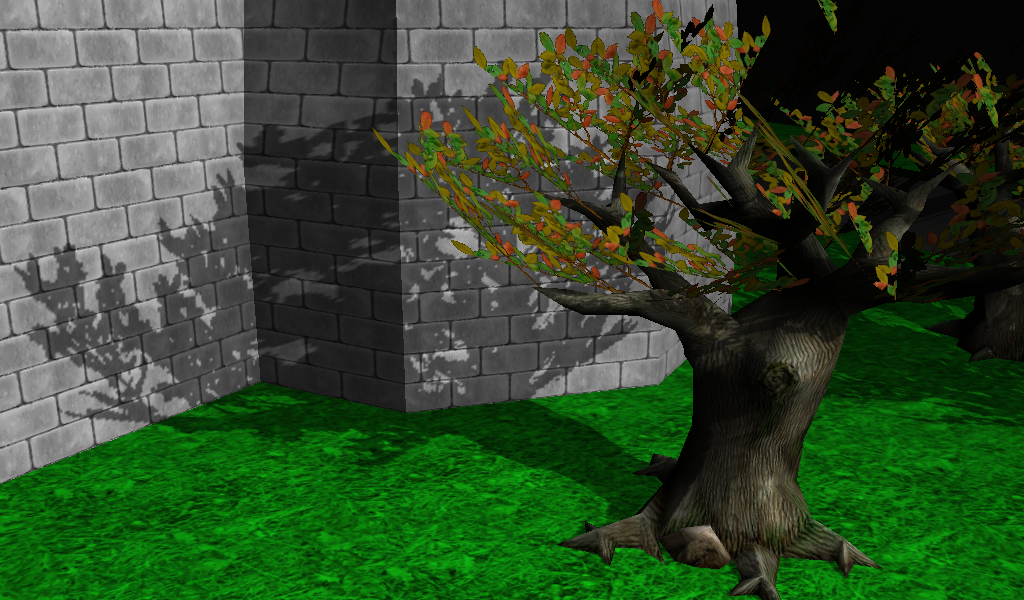
\includegraphics[width=3.0in]{sunny_street_tree_hard}
  \caption{Close up shadows on the tree. Notice that leaves (modeled by alpha-test texture) also cast correct shadows.}
\end{figure}

\section{Shading with the shaders}

When the shape receiving shadows doesn't have any shaders assigned in
the X3D file, we do not require much from the implementation.
We only insist that shadows must be visualized in \emph{some} way,
from at least one shadow map. In the simplest case,
the computed pixel color may be simply set to the pure black
when it falls in the shadow. This way even implementations
for old GPUs, that have only fixed-function pipeline available,
may satisfy our extensions specification.

The encouraged method to make the shadows look nice is to use the shaders.
This way shadows have high-quality look, and the shading doesn't require
any extra rendering passes. The X3D author has full power of customizing
the shadows look when using lower-level \texttt{GeneratedShadowMap}
approach. When the \texttt{receiveShadows} field is used,
browsers are strongly encouraged to use internal shaders for nice shading.

Below we present simple examples how to use GLSL (OpenGL Shading Language)
shaders to make the shadows look nice.
Note that we use GLSL language just as an example. Our extensions
are not OpenGL specific, and any shading language is usable with our shadow maps.
We extend the X3D specification of the shaders component to pass
\texttt{GeneratedShadowMap} to shader's
\texttt{sampler2DShadow} type (for spot and directional
lights) and \texttt{samplerCubeShadow} type (for point lights).
Unless they have \texttt{compareMode} set to \texttt{NONE},
in which case they map (appropriately) to the \texttt{sampler2D} or the \texttt{samplerCube}.
This applies to all shader languages mentioned in the X3D specification:
\emph{OpenGL shading language (GLSL) binding},
\emph{Microsoft high level shading language (HLSL) binding} and
\emph{nVidia Cg shading language binding}.

\subsection{Basics}

In the simplest case, we sample the 2D depth texture using
the \texttt{shadow2DProj(shadowMap, gl\_TexCoord[0])} call.
%%  This is assuming
%% that our depth map is kept in a variable named \texttt{shadowMap},
%% and that the projective texture generator was placed in the first (number 0)
%% texture unit (if using multi-texturing).
A complete GLSL fragment shader looks like this:

%% % Max line length of verbatim is about here:
%% %%%%%%%%%%%%%%%%%%%%%%%%%%%%%%%%%%%%%%%%%%

\begin{mycode}
\begin{Verbatim}
uniform sampler2DShadow shadowMap;
void main(void)
{
  float shadow =
   shadow2DProj(shadowMap, gl_TexCoord[0]).r;
  gl_FragColor = gl_Color * shadow;
  /* add some ambient term */
  gl_FragColor += vec4(0.25, 0.25, 0.25, 1);
}
\end{Verbatim}
\end{mycode}

\begin{figure}[H]
  \centering
  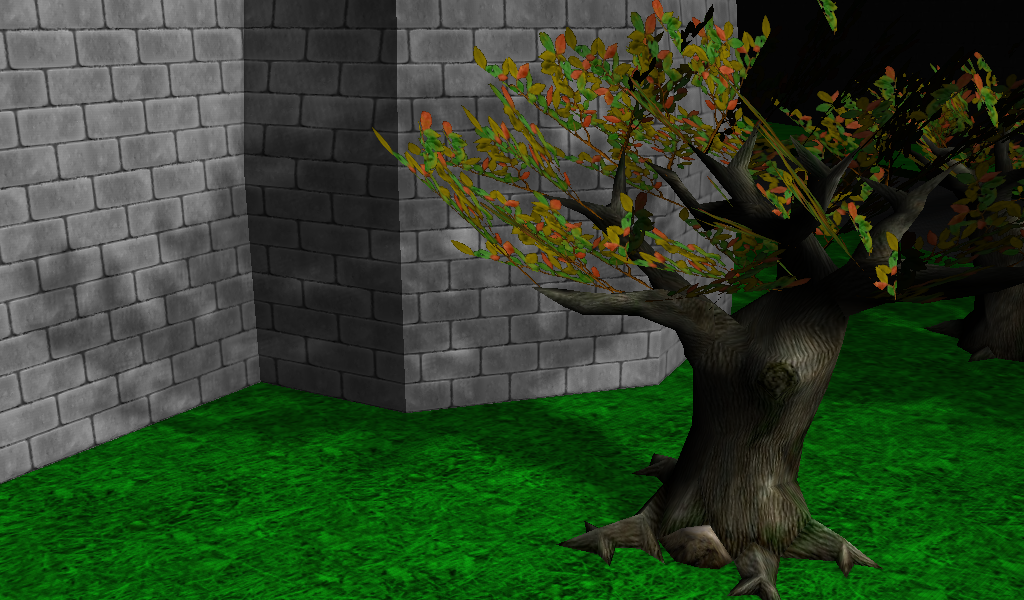
\includegraphics[width=3.0in]{sunny_street_tree_pcf16}
  \caption{The previous tree once again, this time with \textit{percentage closer filtering} (16 samples). Note the soft look of the shadows.}
\end{figure}

This is a very simple shader, and a very crude one. Next we will
describe how to improve it.

\subsection{Improvements}

The shader code in the previous section scales the \texttt{gl\_Color}
value by the shadow amount of a single light. This isn't a correct solution,
as \texttt{gl\_Color} (calculated by the vertex shader or the fixed-function pipeline)
contains the contribution from \emph{all scene lights}.

A better solution would be to calculate the whole lighting inside
the fragment shader
\footnote{Or pass contributions from the separate
lights as separate variables from the vertex shader.}.
Then the \texttt{shadow} value may be used to scale only
the contribution of the appropriate light.
Following this idea, we could also use several shadow maps,
each one from a different light source.
Shader could then calculate lighting with correctly combined shadows
from all the light sources.

Another problem is that the shadow map may be sampled
with positions outside of the $(0, 0) - (1, 1)$ square. This isn't
a problem for spot lights since they do not shine outside of their
cone, so the value of \texttt{shadow} there doesn't matter --- it will
be multiplied by black color anyway. But for directional lights it remains
important. Outside of the $(0, 0) - (1, 1)$ square,
the clamping of the texture coordinates will stretch the shadows over
unrelated scene parts.
We would like to consider everything that is outside of the shadow map
as always in the shadow. This may be done by inserting
(before the \texttt{shadow} value is used in the multiplication)
the following check into the previous shader code:

\begin{mycode}
\begin{Verbatim}
vec2 shadowMapCoord =
  gl_TexCoord[1].st / gl_TexCoord[1].q;
if (shadowMapCoord.s < 0.0 ||
    shadowMapCoord.s > 1.0 ||
    shadowMapCoord.t < 0.0 ||
    shadowMapCoord.t > 1.0)
  shadow = 0.0;
\end{Verbatim}
\end{mycode}

%% For an example and discussion of using GLSL shader with shadow maps,
%% see for example \myhref{http://www.evl.uic.edu/rlk/cs594/final/part3.html}{http://www.evl.uic.edu/rlk/cs594/final/part3.html}.

\subsection{Percentage closer filtering}

\begin{figure*}[b]
  \centering
  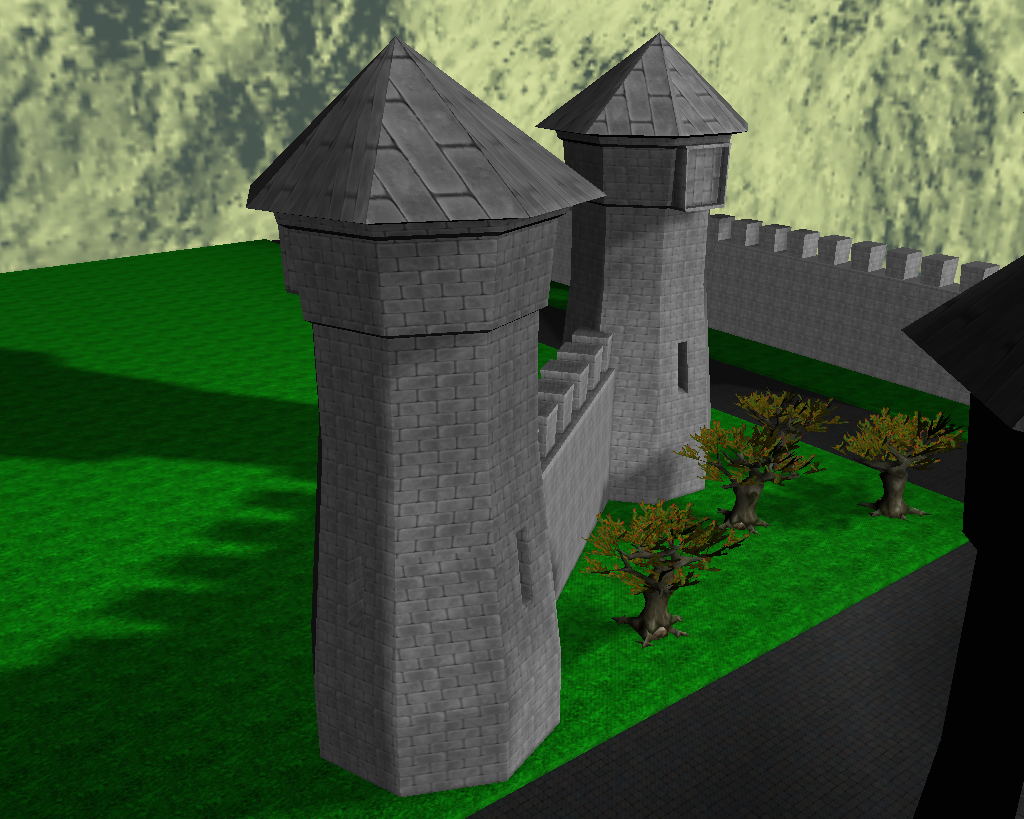
\includegraphics[width=4.0in]{sunny_street_above_view}
  \caption{Yet another screenshot with nice shadow maps.}
\end{figure*}

When the light is far from the shadow receiver, and the user's avatar
looks at the shadow closely, then a single shadow map pixel
corresponds to many pixels on the screen. This means that the shape
of the shadow map pixels is unfortunately visible on the screen.
%% Such aliasing artifacts are (to some extent) unavoidable with shadow maps,
%% since the very idea of shadow maps is to store the shadow information
%% in a texture with a finite size.
\emph{Percentage closer filtering} \cite{gpugems:pcf} hides these artifacts by
averaging
%% a couple of comparison results.
%% The key insight here is that, unlike with ,,normal'' color texture,
%% filtering of the depth texture values makes no sense.
%% These values are distances from the light source to the object,
%% if we average them we will have incorrect distance values
%% (that do not have to correspond to any distance actually occurring in the scene),
%% and moreover we will still have the same aliasing. The solution is
%% to average
the \emph{results} of the shadow tests.
%% , that is the results
%% of \texttt{shadow2DProj} calls.
A trivial implementation inside GLSL shader may be seen here:
\myhref{https://vrmlengine.svn.sourceforge.net/svnroot/vrmlengine/trunk/kambi\_vrml\_test\_suite/x3d/shadow\_maps/shadow\_map\_pcf4.fs}{https://vrmlengine.svn.sourceforge.net/svnroot/vrmlengine/trunk/kambi_vrml_test_suite/shadow_maps/shadow_map_pcf4.fs}.
%% A good hardware may also help here. Modern GPUs may
%% internally filter at least four depth comparison results.

%% An example shader implementing percentage closer filtering with 4 samples:


%% \begin{mycode}
%% \begin{Verbatim}
%% uniform sampler2DShadow shadowMap;
%% void main(void)
%% {
%%   float offset = gl_TexCoord[0].w / 512.0;
%%   gl_FragColor = (
%%     ( shadow2DProj(shadowMap, gl_TexCoord[0] +
%%         vec4(-offset, -offset, 0.0, 0.0)).r +
%%       shadow2DProj(shadowMap, gl_TexCoord[0] +
%%         vec4(-offset,  offset, 0.0, 0.0)).r +
%%       shadow2DProj(shadowMap, gl_TexCoord[0] +
%%         vec4( offset,  offset, 0.0, 0.0)).r +
%%       shadow2DProj(shadowMap, gl_TexCoord[0] +
%%         vec4( offset, -offset, 0.0, 0.0)).r
%%     ) / 4.0 ) * gl_Color;
%% }
%% \end{Verbatim}
%% \end{mycode}

\section{Implementation notes}

An open-source implementation of these extensions is available in our engine on
\myhref{http://vrmlengine.sourceforge.net/}{http://vrmlengine.sourceforge.net/}.
You can test it for example with our \texttt{view3dscene} tool.
An example VRML/X3D files with the shadow maps and the GLSL shaders are available in our test suite
on \myhref{http://vrmlengine.sourceforge.net/kambi\_vrml\_test\_suite.php}{http://vrmlengine.sourceforge.net/kambi_vrml_test_suite.php}
(inside \texttt{x3d/shadow\_maps/} subdirectory).

Our implementation uses the basic OpenGL tools: we render to the depth
texture using the framebuffer object, and we set up projective texturing
by OpenGL \texttt{glTexGen} procedures.
We perform the comparison to determine if the shadows are black by the
\texttt{ARB\_shadow} OpenGL extension.
%% no space: \cite{glext:shadow}.
Everything needed is available in pretty much every sensible OpenGL
implementation (even in the pure software version of Mesa3D).

The case when \texttt{update} is set to \texttt{ALWAYS} is optimized.
The shadow maps are regenerated
only if the geometry of the scene changes. This means that mere camera
movements, or animation of the materials or textures do not cause
an unnecessary update overhead.
An other potential optimization would be to
update shadow maps only once for a couple of frames, or once for
a fraction of a second.

%% The case of \texttt{update="NEXT\_FRAME\_ONLY"}
%% could be actually optimized as well, but for now is not (as it's not important
%% in usual scenarios).

We do not handle shadow maps from \texttt{PointLight} sources yet.

The \texttt{receiveShadows} field is implemented
as a transformation of the X3D nodes graph.
You can try it by the \texttt{view3dscene} menu option
\textit{Handle receiveShadows by shadow maps}.
Currently, the effect of this transformation
may be visible to the author in some uncommon situations,
like when using a script traversing the nodes graph.
%, so it's a small inconvenience.

%% We also do not implement \emph{Perspective Shadow Maps} yet \cite{perspsm}.
%% But their implementation seems possible with no changes to the presented
%% extensions. Note that for perspective shadow maps the optimization
%% of \texttt{update="ALWAYS"} would have to be weakened, as perspective
%% shadow maps depend on the current camera view.

We have also implemented the shadow volumes algorithm \cite{vrmleng:shadowvolumes}
and a software ray-tracer.
They both honor the \texttt{shadowCaster} field.
Our ray-tracer treats everything as a shadow receiver.
Our current shadow volumes implementation is slightly limited,
and requires special lights setup,
also treating everything as a shadow receiver.
Non-manifold shadow casters are detected but currently still
used by the shadow volumes implementation --- this is useful for special
non-manifold shapes in some scenes,
at the risk of showing ugly artifacts from particular camera angles.

\section{Conclusion}

We have presented a number of extensions to the existing X3D specification.
Together, they allow the authors to control the shadow maps
behavior on the 3D scenes.
Authors can also use projective texturing
as an independent feature, for example to cast normal colored textures
from the light sources or viewpoints. Generated shadow map textures can be also
visualized as a grayscale 2D textures, which is very useful for debugging
shadow map depth problems.

Most important (and scene-dependent) parameters
of the shadow map generation can be set in the X3D code, while the implementation
is delegated to hide most of the dirty work. Natural implementation
in both fixed-function and shader pipelines is possible. Shadow maps
defined this way cooperate nicely with user's custom shader code.

%\needspace{1in}
\section{Future work}

%% \subsection{Allow browser internal shaders to cooperate with custom shaders}

Shadow mapping, as well as many other effects,
would benefit from X3D browser being able to use it's own
internal shader code.
For example, advanced bump mapping variants
(like \emph{steep parallax bump mapping with self-shadowing} \cite{parallaxbump})
can be sensibly implemented only using the shaders.
Current implementation of the bump mapping extension in our engine
forces the author to make a difficult choice:
\emph{either} easily ,,turn on the bump mapping'' (our bump mapping extensions
require only to provide the height and normal maps \cite{vrmleng:parallaxbump}) and resign
from custom shaders \emph{or} resign from using our comfortable
extensions and implement bump mapping yourself with own shaders.
The simple \texttt{receiveShadows} extension described in the section
\ref{sec_receive_shadows} has the same disadvantage: browser's internal shaders
have to override author's custom shaders in this case.

It's worth exploring how to merge such systems. Ideally, author should be able
to write his own shader code, and at the same time the implementation
must be able to implement some effects through internal shaders.
Author must have the ability to selectively use or override
all the effects of the browser.

A flexible approach to cooperate between user and browser shader code
(preferably an approach mapping to the various shader languages:
GLSL, Cg, HLSL, also CgFX) seems like a mighty extension for X3D.

\section*{Acknowledgements}

The author would like to thank the many people that encouraged the development
and helped to test our VRML/X3D engine. In particular Victor Amat
was experimenting with \emph{Screen Space Ambient Occlusion}
and uncovered many quirks in the implementation.

Andrzej {\L}ukaszewski did the proofreading of this paper and suggested
a lot of the improvements.

The 3D scenery with trees and towers visible on many screenshots in this paper
was constructed with the help of the assets from \myhref{http://opengameart.org}{http://opengameart.org},
a great site with good quality 3D assets on clear open-source licenses.
See the \myhref{https://vrmlengine.svn.sourceforge.net/svnroot/vrmlengine/trunk/vrml\_engine\_doc/shadow\_maps\_x3d/sunny\_street/}{https://vrmlengine.svn.sourceforge.net/svnroot/vrmlengine/trunk/papers/shadow_maps_x3d/sunny_street/}
for the full scene code in X3D, helper transformation program and the
\texttt{README.txt} file with detailed credits.

%% The folks at
%% \myhref{http://www.nvidia.com/}{http://www.nvidia.com/}
%% also deserve a mention, for publishing a lot of material
%% General thanks to eveyone that helped with the VRML/X3D standards development.
%% Thanks!

\bibliographystyle{acmsiggraph}
\nocite{*}
\bibliography{shadow_maps_x3d}

\end{document}
